\documentclass[a4paper]{article}
\usepackage[left=1cm, right=1cm, top=1cm, bottom=1cm]{geometry}
\usepackage{amsmath}
\usepackage{amssymb}
\usepackage{amsfonts}
\usepackage{subcaption}
\usepackage{caption}
\usepackage{graphicx}
\usepackage{fullpage}
\usepackage{textcomp}
\usepackage{listings}
\usepackage{xcolor}
\usepackage{float}
\usepackage[toc,page]{appendix}

% hyperref must be last
\usepackage{hyperref}
\hypersetup{
  backref=true,
  colorlinks=true,
  linkcolor=blue,
  citecolor=blue,
  urlcolor=blue
}
\lstset{ 
  language=Matlab, % choose the language of the code
  basicstyle=\fontfamily{pcr}\selectfont\footnotesize\color{black},
  keywordstyle=\color{red}\bfseries, % style for keywords
  numbers=none, % where to put the line-numbers
  numberstyle=\tiny, % the size of the fonts that are used for the line-numbers
  %  keywordstyle     = \bfseries,
  identifierstyle  = \color{blue},
  commentstyle     = \color{olive},     
  backgroundcolor=\color{white},
  showspaces=false, % show spaces adding particular underscores
  showstringspaces=false, % underline spaces within strings
  showtabs=false, % show tabs within strings adding particular underscores
  frame=single, % adds a frame around the code
  tabsize=2, % sets default tabsize to 2 spaces
  rulesepcolor=\color{gray},
  rulecolor=\color{black},
  captionpos=b, % sets the caption-position to bottom
  breaklines=true, % sets automatic line breaking
  breakatwhitespace=false, 
}
\title{Shape Optimization of Wind Spar Under Uncertainty}
\author{ID:4873}
\begin{document}
 \maketitle
 
\begin{abstract}
   In this project we design the shape of a wing spar under uncertainty using numerical optimization techniques such that given total weight of an aircraft and material property, and certain uncertainty in the loading, the weight of the spar is minimized. Compared to the second project which is deterministic, this problem is challenging due to the presence of uncertainty in the loading. The core problem involves how the uncertainty in the loading propagate to the stress which serves as constraints in the optimization problem. The approach employed in this work is the stochastic collocation. We will focus on the uncertainty analysis and the optimization under uncertainty. At the end, results and conclusion are given.
\end{abstract}

\section{Physics Model} \label{sec:physics}
The wind spar is used to support the aerodynamic force acting on the aircraft. The cross-section shape of the spar in this project is a circular annulus, with size constraints as follows
\begin{equation}
\begin{aligned}
r &\ge 0.02m \\
R &\le 0.05m \\
R-r &\ge 0.0025m\\
\end{aligned}
\end{equation}
where $r$ and $R$ are the inner and outer radius of the circular annulus, respectively.
The spar is made of carbon fiber composite, with density $1600\:km/m^3$, Young's modulus $70\:GPa$, and ultimate tensile/compressive strength $600\: MPa$.

The loading on the spar is defined as follows
\begin{equation}
f(x,\xi) = f_{nom}(x) + \delta_{f}(x,\xi)
\end{equation}
where the nomial loading is given by
\begin{equation}
f_{nom}(x) = \frac{2.5W}{L}(1-\frac{x}{L})
\end{equation}
and the probabilistic perturbation $\delta_{f}$ has the form
\begin{equation}
\delta_{f}(x,\xi) = \sum_{n=1}^{4}\xi_n \cos(\frac{(2n-1)\pi x}{2L})
\end{equation}
 $2.5$ times the weight of the aircraft, and the force is assumed to be linearly distributed, with maximum load at the root and zero load at the tip.

The objective is to minimize the weight of the spar without a combination of the mean value and standard deviations of the stress reaching the ultimate strength of the carbon fiber:
\begin{equation}
\sigma_{un} = E[\sigma(x,\xi)] + 6\sqrt{Var[\sigma(x,\xi)]} \le s_{yield}
\end{equation}
\section{Mathematical Model}
\subsection{Optimization problem}
To use an numerical optimization technique, the physics model in Section~\ref{sec:physics} must be rewritten into a mathematical model. The one used in this work is as follows:
\begin{equation} \label{eq:math_model_1}
\begin{aligned}
max\:\: &f(r(x), R(x)) \\
s.t.\:\: & r(x) \ge 0.02 \\
         & R(x) \le 0.05 \\
         & R(x)-r(x) \ge 0.0025 \\
         &\sigma_{un}(r(x), R(x)) \le \sigma_{yield}
\end{aligned}
\end{equation}
where $\sigma_{yield}$ is ultimate strength of the fiber, $f$, the objective function, is the weight of the spar, 
\begin{equation*}
f = \int \pi (R^2 - r^2) dx
\end{equation*}
and $\sigma$ the stress of the spar subject to the loading. The relation between the stress and the shape of the spar ($r$ and $R$) is governed by the Euler-Bernoulli beam equation:
\begin{equation}\label{pde}
\begin{aligned}
{\cfrac  {\partial ^{2}}{\partial x^{2}}}\left(EI{\cfrac  {\partial ^{2}w}{\partial x^{2}}}\right)=q(x)\\
\sigma =-zE~{\frac  {{\mathrm  {d}}^{2}w}{{\mathrm  {d}}x^{2}}}
\end{aligned}
\end{equation}
where $q$ is the loading force, $E$ the Young's modulus, $I$ the second moment of area, $w$ the the deflection of the spar. In this specific problem, the linearly distributed force $q=500*2.5*9.8/L (1-x/L)$.

See \url{https://en.wikipedia.org/wiki/Euler%E2%80%93Bernoulli_beam_theory} for more infomation on the Euler-Bernoulli beam theory.


\section{Analysis model} \label{sec:analysis_tool}
\subsection{Shape optimization}\label{shape_param}
The shape parameterization used here is a weighted summation of monomials:
\begin{equation}
\begin{aligned}
r(x) &= \sum_{i=1}^{N_{var}/2} a_ix^{i-1}\\
R(x) &= \sum_{i=1}^{N_{var}/2} a_{i+N_{var}/2}x^{i-1}
\end{aligned}
\end{equation}
where $a_i$ is the design variable, and $N_{var}$ is the number of design variables.
\subsection{Finite element solver}
In order to compute the stress appearing in the inequality constraints in \eqref{eq:math_model_1}, we need to solve the differential equation \ref{pde}. In this project, the Euler-Bernoulli equation \eqref{pde} is solved with finite element methods.


\section{Implementation}
The implementation in Matlab is attached in Appendix~\ref{app:calcweight}$\sim$\ref{app:new_const2}. 

\subsection{Objective function and its gradient, geometric constraints}\label{sec:obj}
The objective function and its derivative and geometric constraints remain unchanged from project-2.


\subsection{Nonlinear constraints}
This nonlinear constraints are realized in two steps:
\begin{itemize}
  \item first, we define a function
  
  \hspace{10 mm}\texttt{function [mean\_cineq, sigma\_cineq] = calcMeanAndStandardDeviationOfStress ( L, E, force, x, a )}\\
  to compute the mean value and standard deviation of the stress under uncertainty. The Guass-Hermite quadrature ruls is used to compute the mean value. The old function from project-2 \\
  \texttt{function [mean\_cineq, sigma\_cineq] = calcMeanAndStandardDeviationOfStress ( L, E, force, x, a )}\\
   is called. This is realized in Appendix~\ref{app:new_const}
  \item then, the new nonlinear constraints is defined as a combination of \texttt{mean\_cineq} and \texttt{sigma\_cineq}. This is realized in Appendix~\ref{app:new_const2}
\end{itemize}

\section{Results and discussion}
12 cases were run to study the performance of current method, with the order of monomial basis from $1\sim 4$, and 3 different grids. In all cases the same initial shape is specified which corresponds to linear $r=0.04635$ and $R=0.05$ with $f_{init} = 1.325793e+01$. Besides, we use 3 quadrature points for all cases. 

Figure.~\ref{fig:final_shape} show the inner and outer shape of the circular annulus. Table~\ref{tb:weight} and~\ref{tb:weight_old} list the optimized weight of the spar with and without uncertainty. We can see that under uncertainty, the optimized weights for all cases under uncertainty are slightly higher that their deterministic counterparts. $46.29\% \sim 62.20\%$ reduction in weight is achieved after the design.

Besides, as can be seen in Table~\ref{tb:weight}, with the same basis in shape parameterization, the weight of the spar does not change significantly as the number of elements is increased. However, from Figure.~\ref{fig:final_shape} we can see that for monomial order of $3\sim 4$, the final shapes are significantly different from grid to grid.
On the other hand, the results heavily depend on the order of the basis. Specifically, the higher the order of the basis, the smaller the optimized weight.

Figure.~\ref{fig:mean} and Figure.~\ref{fig:deviation} show the mean value of the stress and the standard deviation of the stress at the final step with the finest grid. As can been seen, in spite of difference in the magnitude, both mean value and the standard deviation show similar patterns.

\begin{table}[h]
  \begin{center}
    \caption[]{Optmized weight of spar under uncertainty} \label{tb:weight}
    \begin{tabular}{p{0.05\textwidth}p{0.15\textwidth}p{0.15\textwidth}p{0.15\textwidth}}
      \hline
      order&      nElems=5  & nElems=10   & nElems=20 \\
      \hline
      1&          7.08825 &  7.11313&    7.1209 \\
      2&          5.66483 &  5.72325 &   5.75916  \\
      3&          5.20505&   5.22165&     5.24278    \\
      4&          5.0111&   5.22468&     5.3536\\
      \hline
    \end{tabular}
  \end{center}
\end{table}
\begin{table}[h]
  \begin{center}
    \caption[]{Deterministic optmized weight of spar} \label{tb:weight_old}
    \begin{tabular}{p{0.05\textwidth}p{0.15\textwidth}p{0.15\textwidth}p{0.15\textwidth}}
      \hline
      order&      nElems=5  & nElems=10   & nElems=20 \\
      \hline
      1&          7.087691e+00 &  7.112617e+00 &   7.120396e+00  \\
      2&          5.664373e+00 &  5.719084e+00&    5.755517e+00 \\
      3&          5.175438e+00&   5.222951e+00&     5.241904e+00    \\
      4&          5.000245e+00&   5.037060e+00&     5.066670e+00\\
      \hline
    \end{tabular}
  \end{center}
\end{table}


\begin{figure} [H]
  \begin{subfigure}{0.445\textwidth}
    \centering
    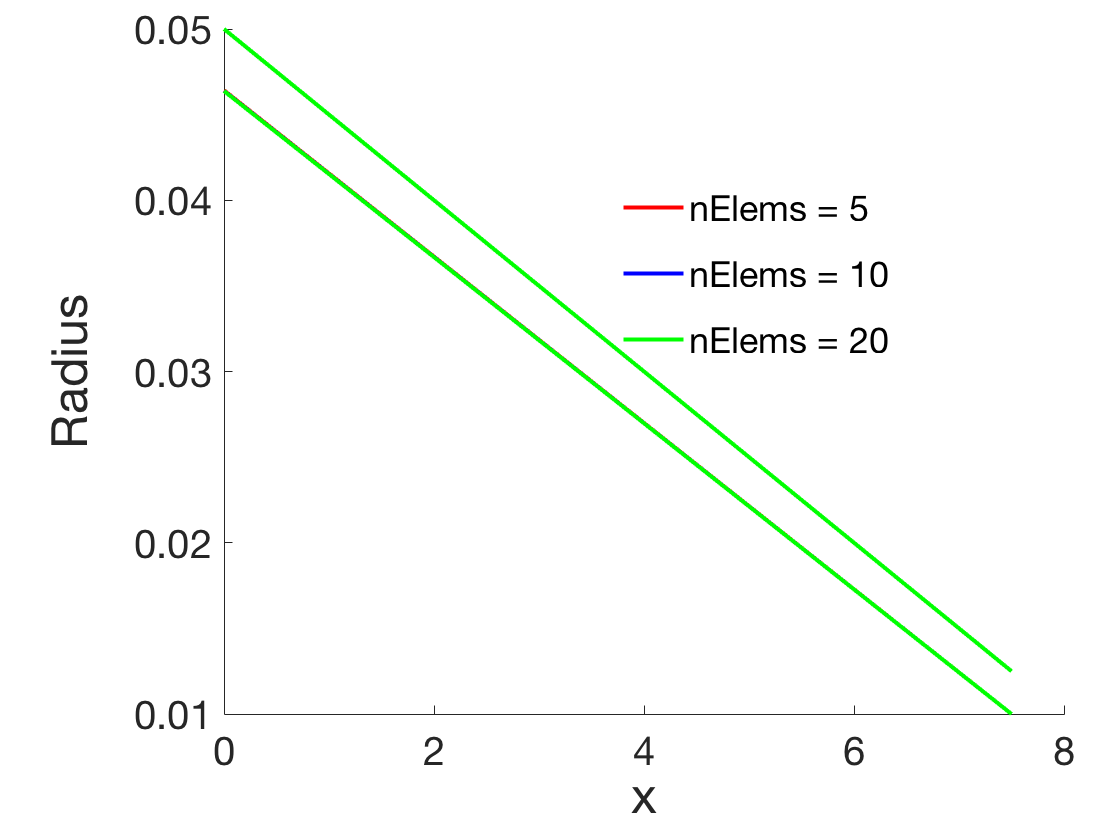
\includegraphics[width=1.0\linewidth]{p1.png}
    \subcaption{linear}
    \label{fig:linear}
  \end{subfigure}
  \begin{subfigure}{0.45\textwidth}
    \centering
    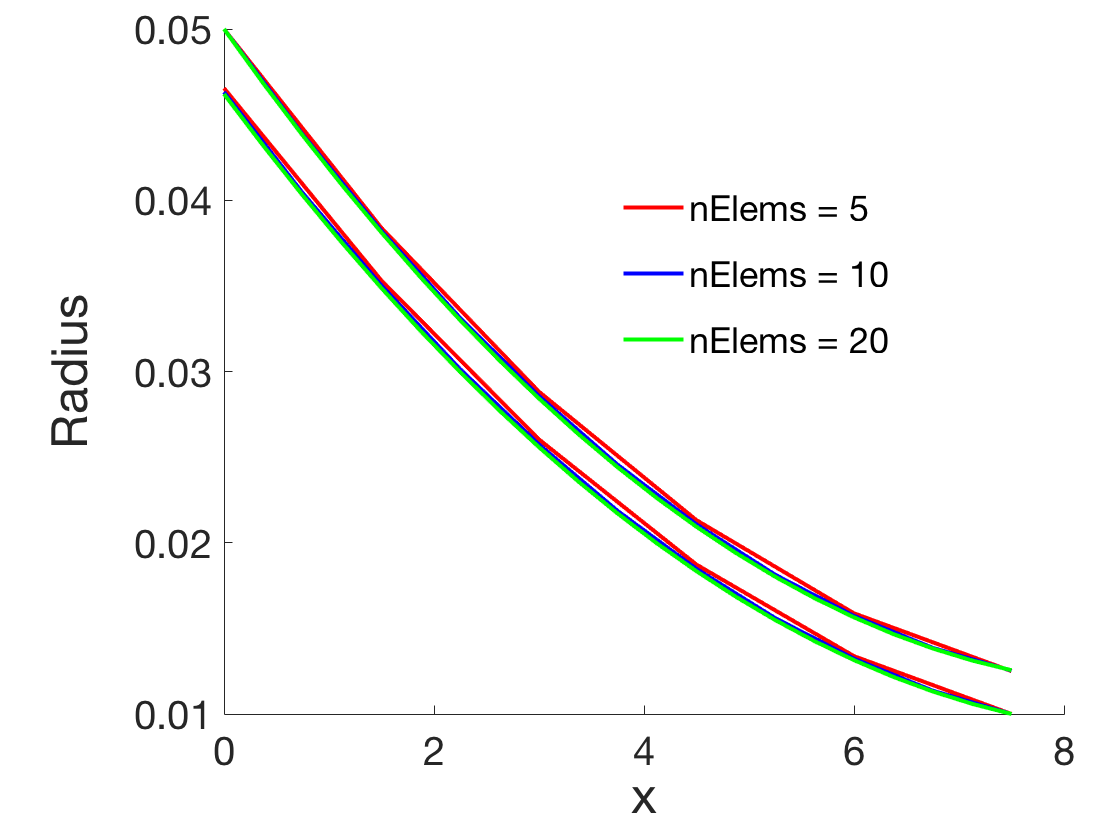
\includegraphics[width=1.0\linewidth]{p2.png}
    \subcaption{quadratic}
    \label{fig:quadratic}
  \end{subfigure}\\[4ex]
  \begin{subfigure}{0.45\textwidth}
    \centering
    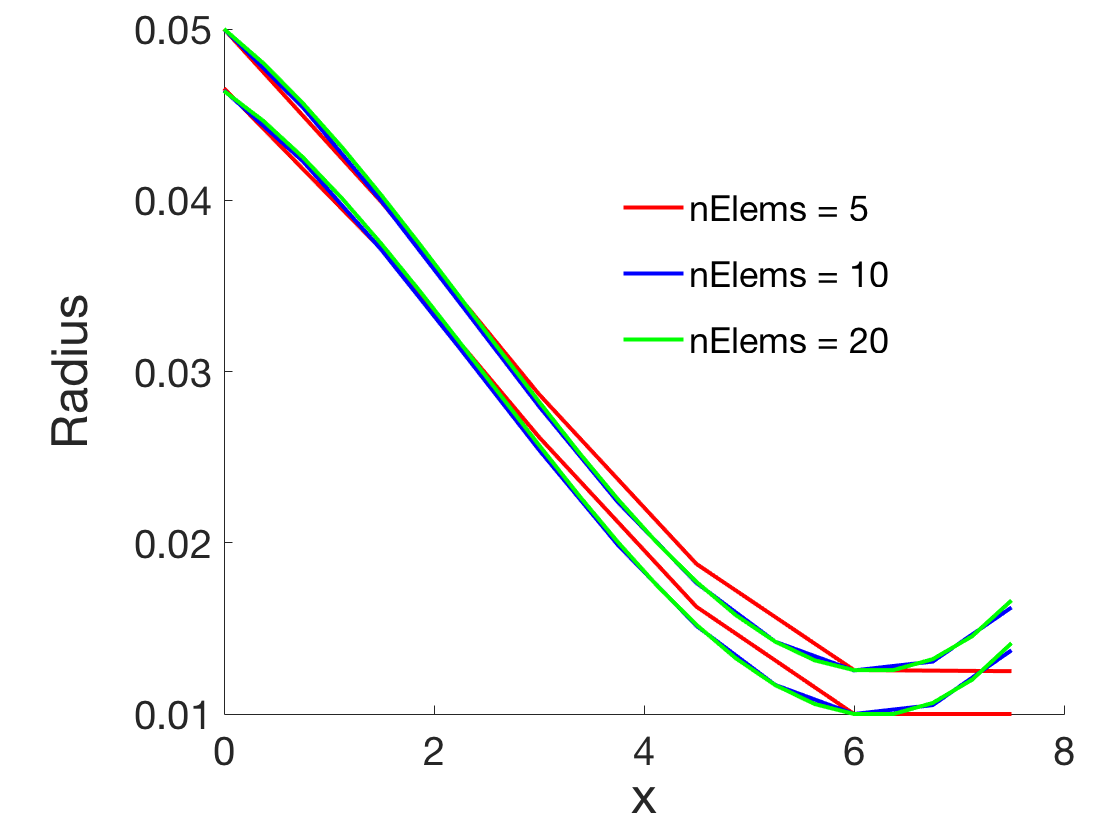
\includegraphics[width=1.0\linewidth]{p3.png}
    \subcaption{cubic}
    \label{fig:cubic}
  \end{subfigure}
  \begin{subfigure}{0.45\textwidth}
    \centering
    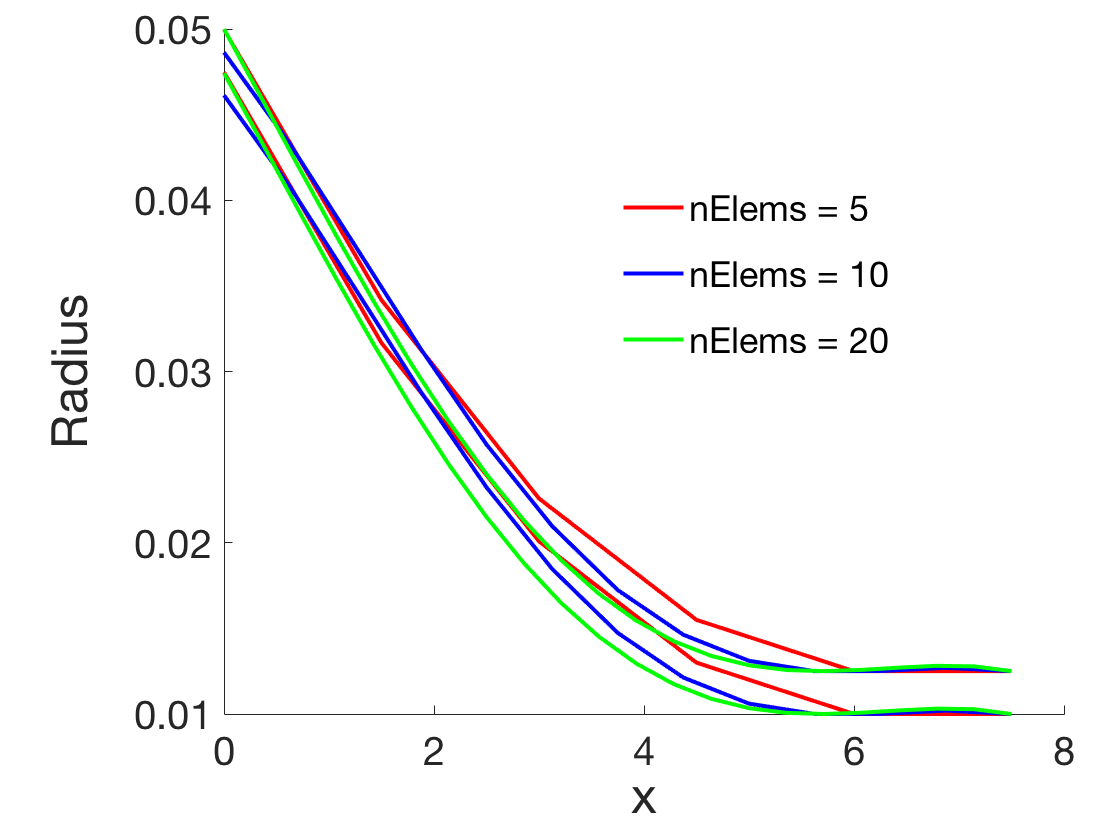
\includegraphics[width=1.0\linewidth]{p4.png}
    \subcaption{quartic}
    \label{fig:quatic}
  \end{subfigure}  
  \caption{Optimized shape of circular annulus  \label{fig:final_shape}}
\end{figure}

\begin{figure} [H]
  \begin{subfigure}{0.45\textwidth}
    \centering
    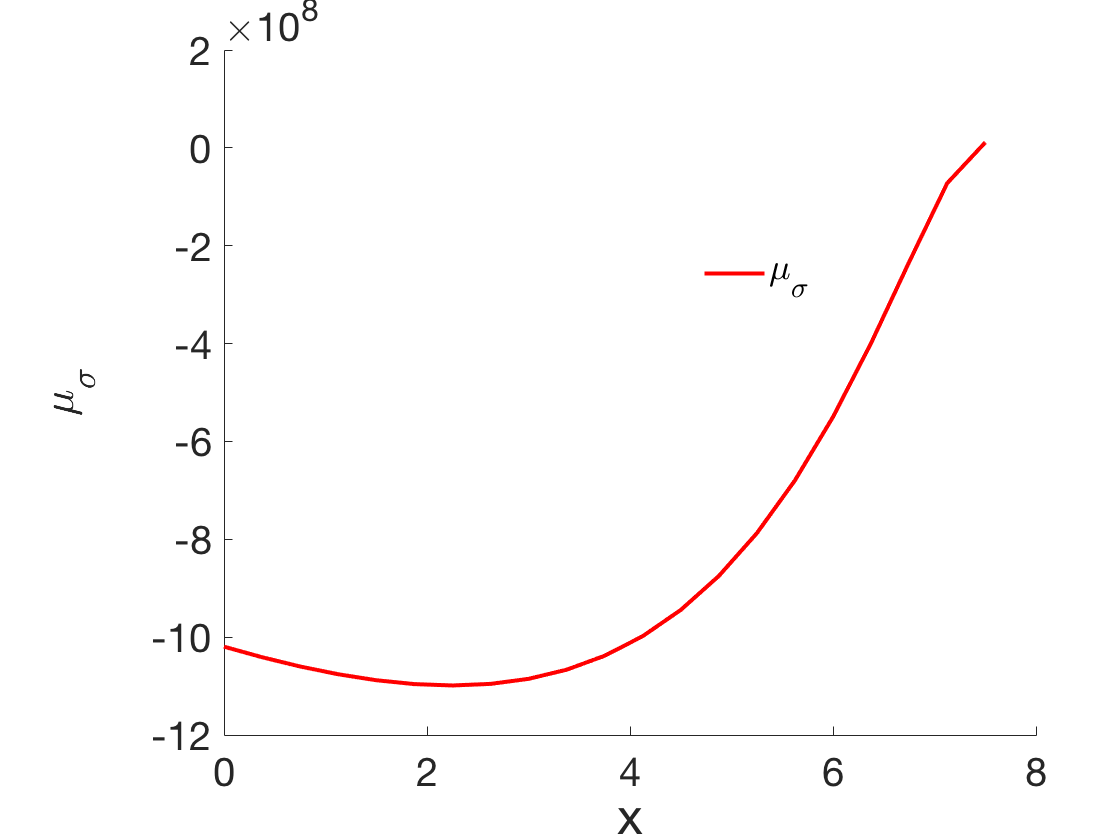
\includegraphics[width=1.0\linewidth]{p1n20_mean.png}
    \subcaption{linear}
    \label{fig:mean_p1}
  \end{subfigure}
  \begin{subfigure}{0.45\textwidth}
    \centering
    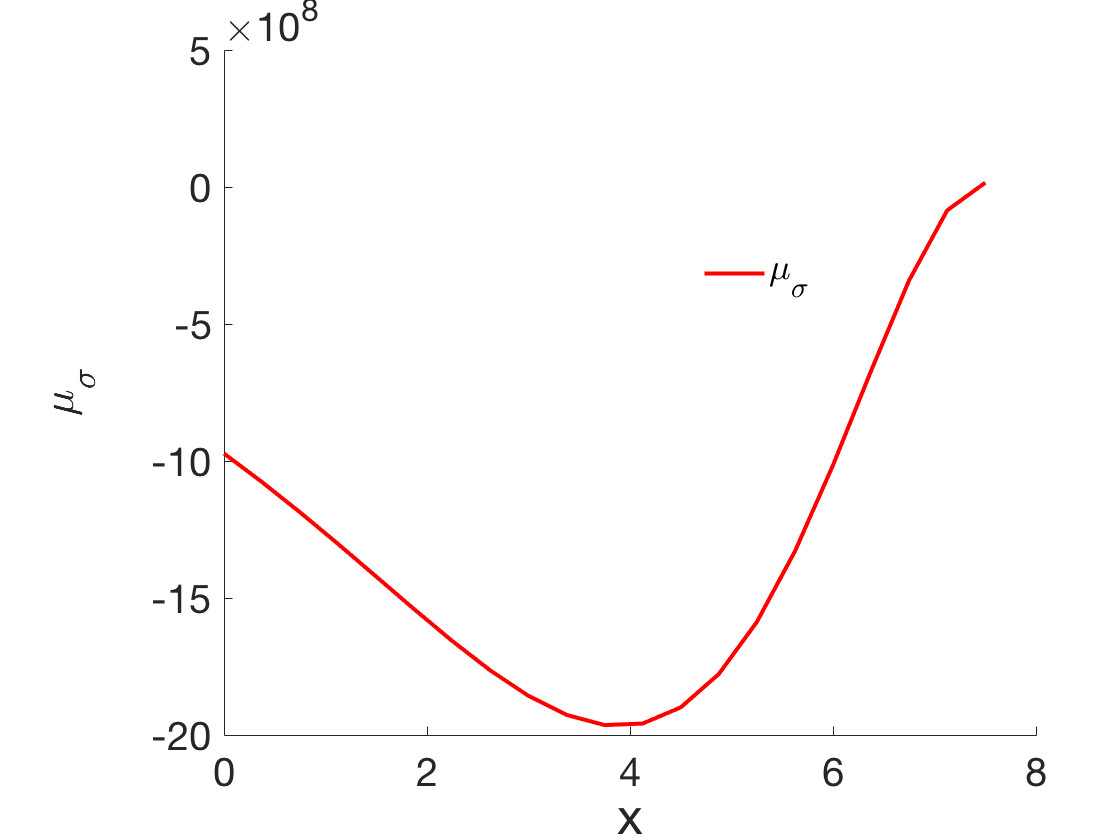
\includegraphics[width=1.0\linewidth]{p2n20_mean.png}
    \subcaption{quadratic}
    \label{fig:mean_p2}
  \end{subfigure}\\[4ex]
  \begin{subfigure}{0.45\textwidth}
    \centering
    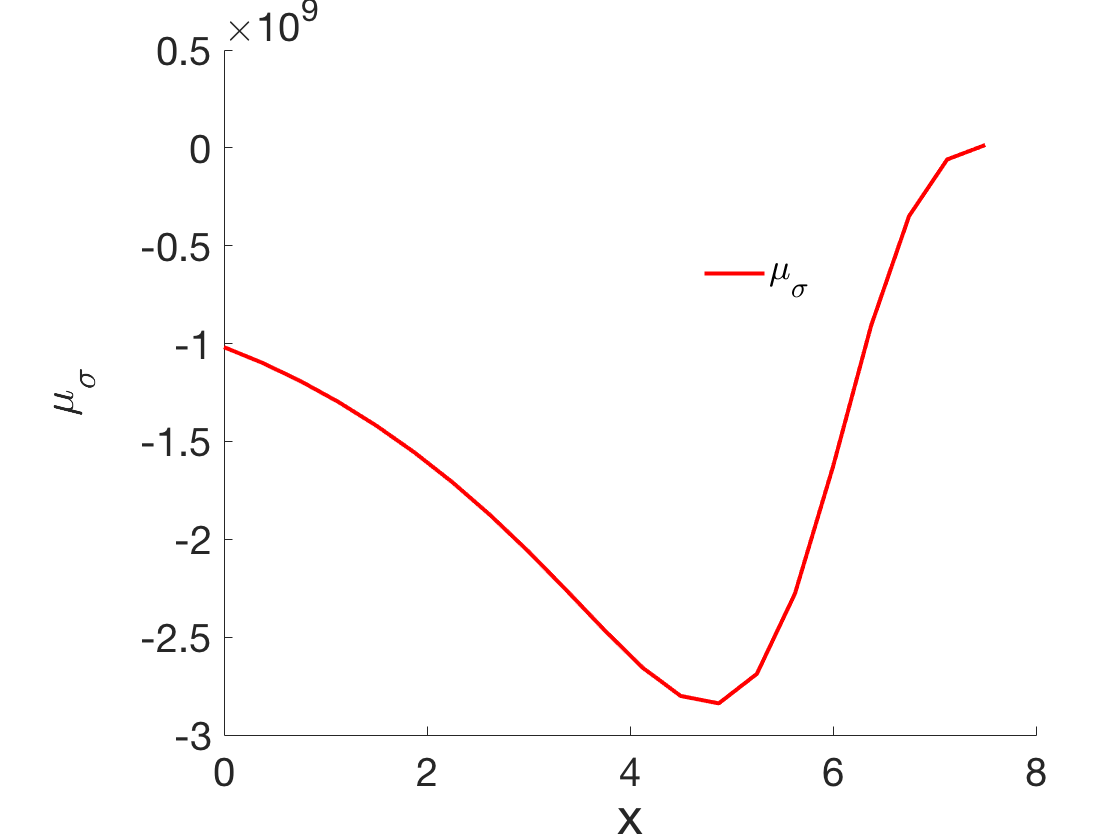
\includegraphics[width=1.0\linewidth]{p3n20_mean.png}
    \subcaption{cubic}
    \label{fig:mean_p3}
  \end{subfigure}
  \begin{subfigure}{0.45\textwidth}
    \centering
    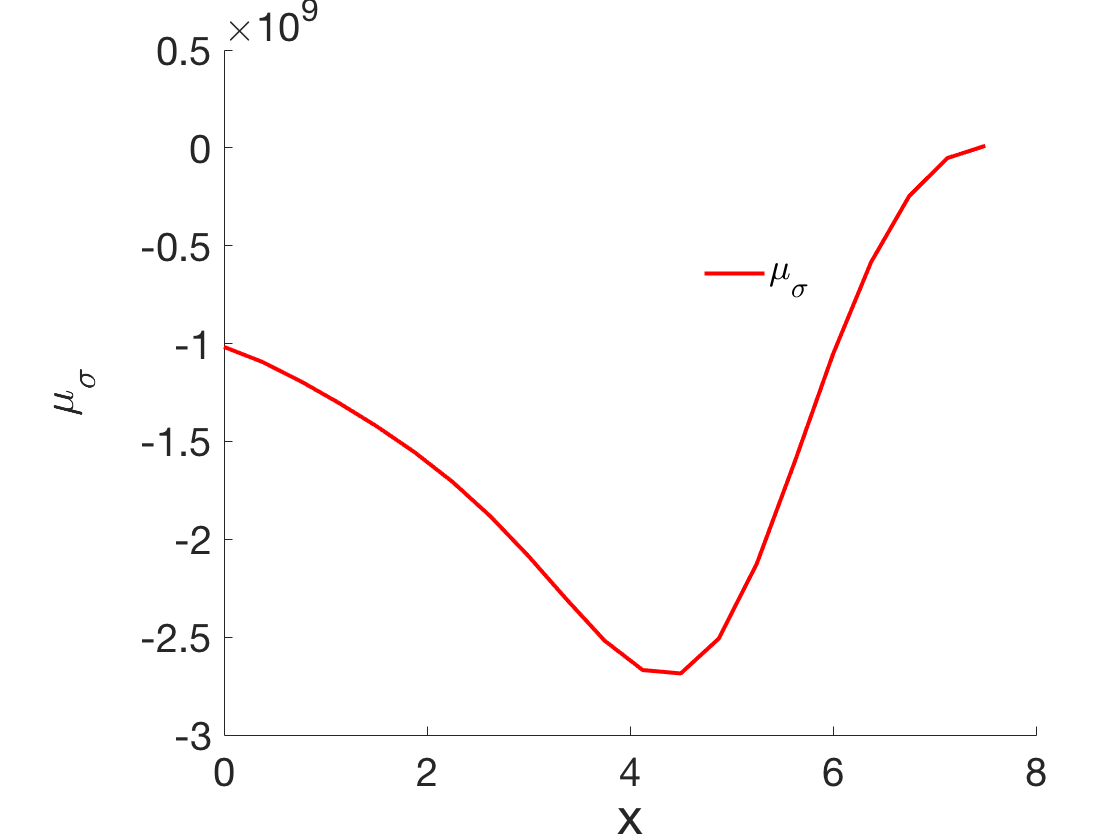
\includegraphics[width=1.0\linewidth]{p4n20_mean.png}
    \subcaption{quartic}
    \label{fig:mean_p4}
  \end{subfigure}  
  \caption{Mean value of stress after convergence, \texttt{nElems = 20} \label{fig:mean}}
\end{figure}
\begin{figure} [H]
  \begin{subfigure}{0.45\textwidth}
    \centering
    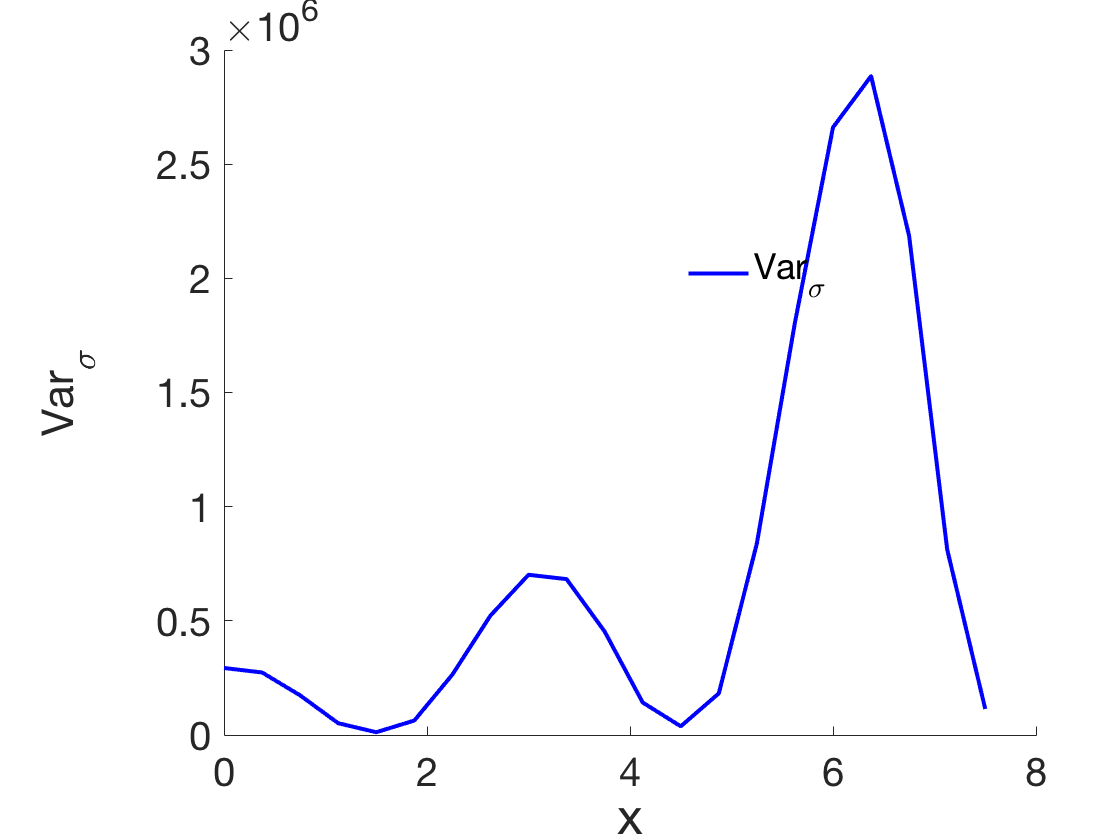
\includegraphics[width=1.0\linewidth]{p1n20_deviation.png}
    \subcaption{linear}
    \label{fig:deviation_p1}
  \end{subfigure}
  \begin{subfigure}{0.45\textwidth}
    \centering
    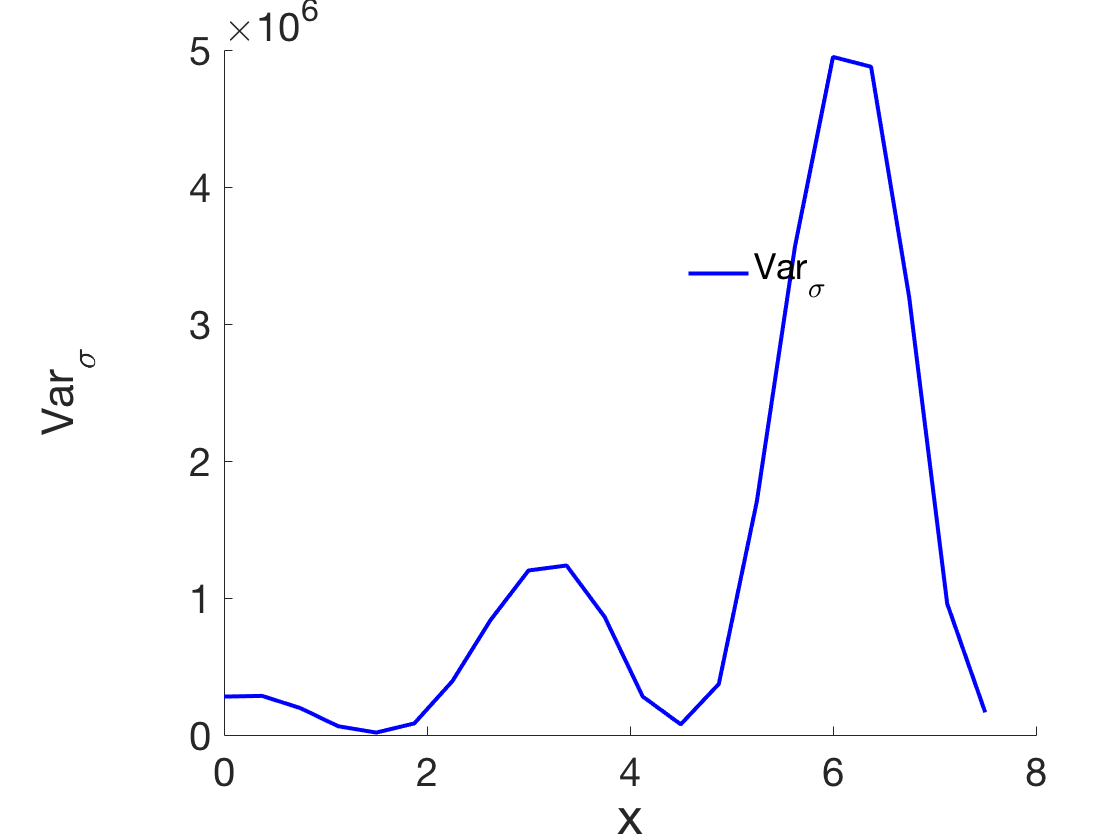
\includegraphics[width=1.0\linewidth]{p2n20_deviation.png}
    \subcaption{quadratic}
    \label{fig:deviation_p2}
  \end{subfigure}\\[4ex]
  \begin{subfigure}{0.45\textwidth}
    \centering
    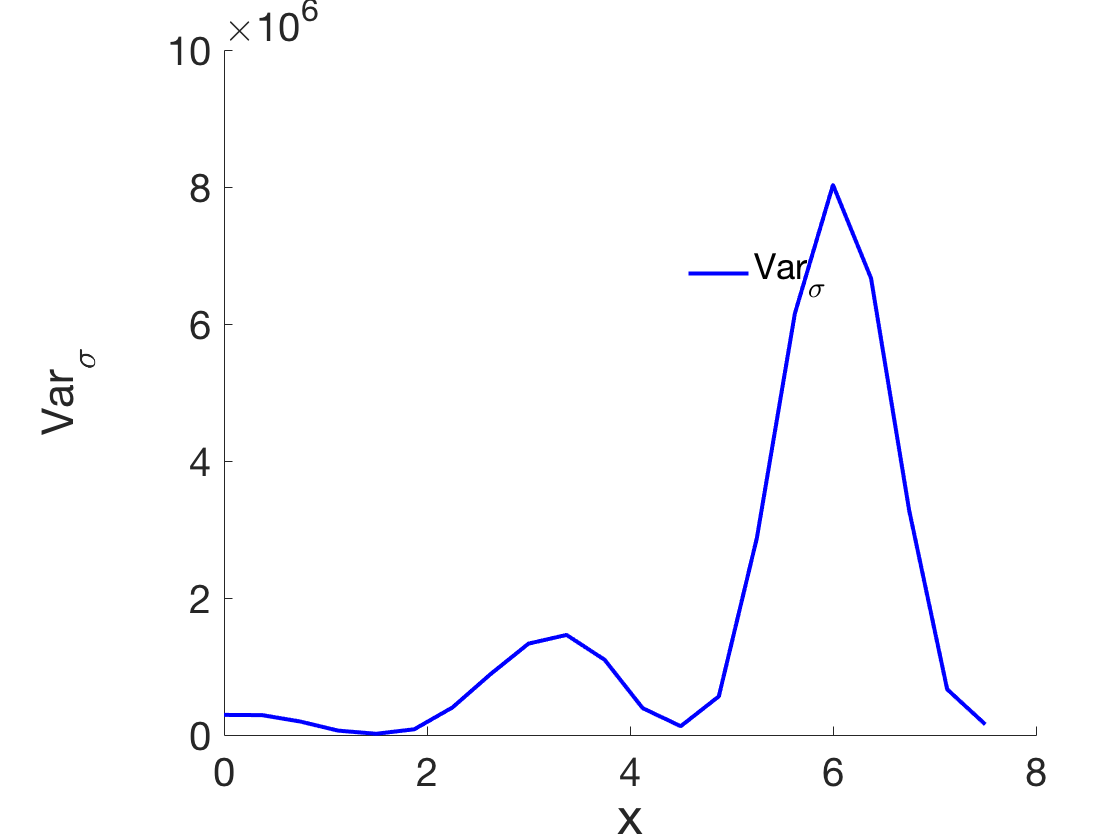
\includegraphics[width=1.0\linewidth]{p3n20_deviation.png}
    \subcaption{cubic}
    \label{fig:deviation_p3}
  \end{subfigure}
  \begin{subfigure}{0.45\textwidth}
    \centering
    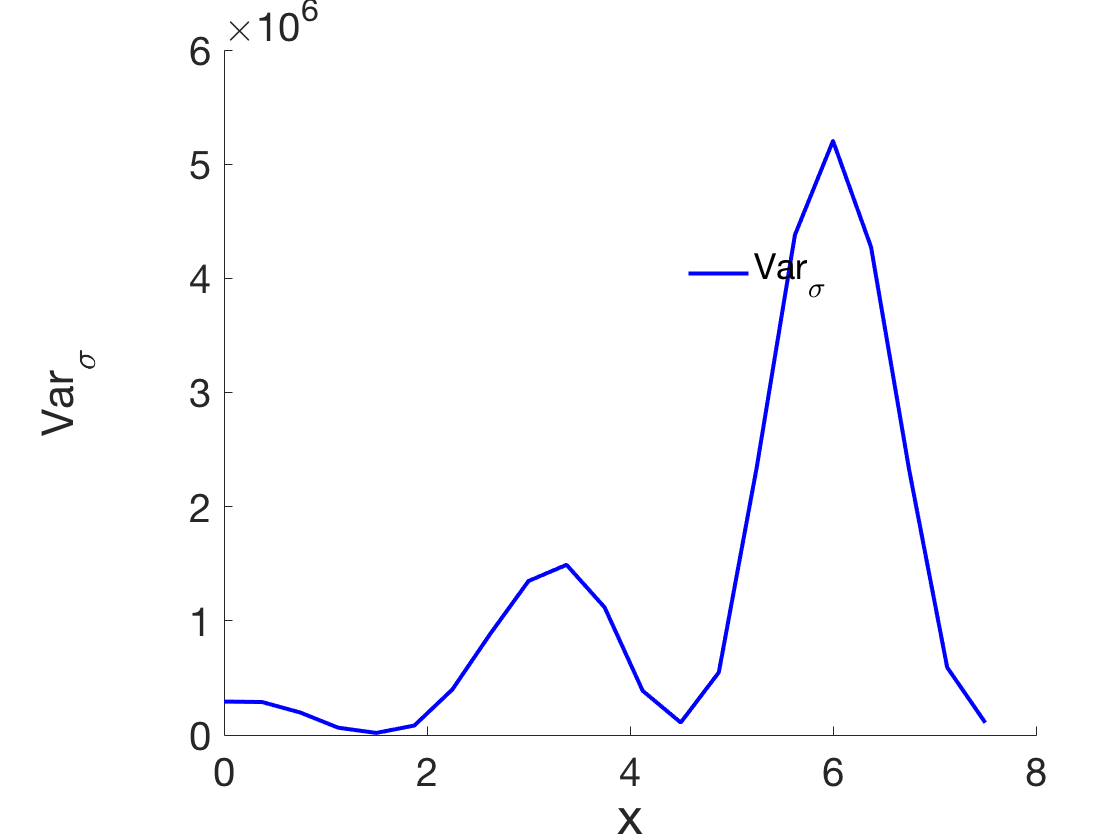
\includegraphics[width=1.0\linewidth]{p4n20_deviation.png}
    \subcaption{quartic}
    \label{fig:deviation_p4}
  \end{subfigure}  
  \caption{Standard deviation of stress after convergence, \texttt{nElems = 20} \label{fig:deviation}}
\end{figure}

\section{Conclusion}
In this work, we use numerical optimization design technique to reduce the weight of a wing spar with loading under uncertainty. The mean value of stress is calculated using stochastic collocation method in conjunction with Gauss-Hermite quadrature rule. The results see significant reduction in spar weight, which proves the effective the current methods.

\small
\begin{appendices} 
\section{calcWeight.m}\label{app:calcweight}
\begin{lstlisting}[language=Matlab]
function [ weight ] = calcWeight( x, a )
%
% Calculate the weight of spar
%
density = 1600;
nElems = size(x, 1) - 1;
% get inner and outer radii
[r, R] = geomParameterization(x, a);
% loop over all elements, accumulate the volume
weight = 0.0;
for i = 1 : nElems
  dx = x(i+1) - x(i);
  area = R(i+1)*R(i+1) - r(i+1)*r(i+1) + R(i)*R(i) - r(i)*r(i);
  weight = weight + area * dx;
end
% factor pi comes from S = pi*R^2; 
% factor 0.5 comes from average of bottom and top area of each element.
weight = weight * 0.5 * pi * density;
end

\end{lstlisting}

\section{calcWeightDerivative.m}\label{app:calcweightderiv}
\begin{lstlisting}[language=Matlab]
function [ dwda ] = calcWeightDerivative( x, a )
%
% complex-variable method to compute the gradient of weight
% w.r.t the design variable.
%
nVars = size(a, 1);
dwda = zeros(nVars, 1);
eps = 1.0e-12;
for i = 1 : nVars
  a(i) = a(i) + complex(0.0, eps);
  weight = calcWeight(x, a);
  dwda(i) = imag(weight) / eps;
  a(i) = a(i) - complex(0.0, eps);
end
end

\end{lstlisting}

\section{objFunc.m}\label{app:calcobj}
\begin{lstlisting}[language=Matlab]
function [ cineq, ceq, dcineq_da, dceq_da] ...
      = calcIneqConstraints( L, E, force, x, a, dcineq_da_old, dceq_da_old)
[cineq, ceq] = calcMeanStressConstraints(L, E, force, x, a);
if nargout > 2 
  dcineq_da = dcineq_da_old;
  dceq_da = dceq_da_old;
end
end

\end{lstlisting}

\section{calcIneqDerivative.m}\label{app:nonconderiv}
\begin{lstlisting}[language=Matlab]
function [ dcineq_da, dceq_da ] = calcIneqDerivative( L, E, force, x, a )
%
% complex-variable method to compute the derivative of inequality
% function w.r.t. design variable a
%
[cineq, ceq] = calcStressConstraints(L, E, force, x, a);
nVars = size(a, 1);
nineq = size(cineq, 1);
neq   = size(ceq, 1);
dcineq_da = zeros(nVars, nineq);
dceq_da   = zeros(nVars, neq);
eps = 1.0e-12;

for i = 1 : nVars
  a(i) = a(i) + complex(0.0, eps);
  [cineq, ceq] = calcStressConstraints(L, E, force, x, a);
  a(i) = a(i) - complex(0.0, eps);
  for j = 1 : nineq
    dcineq_da(i, j) = imag(cineq(j)) / eps;
  end
  for j = 1 : neq
    dceq_da(i, j) = imag(ceq(j)) / eps;
  end
end
end
\end{lstlisting}

\section{calcStressConstraints.m}\label{app:nonlcon}
\begin{lstlisting}[language=Matlab]
function [ cineq, ceq, dcineq_da, dceq_da ] ...
    = calcIneqConstraints( L, E, force, x, a )
[cineq, ceq] = calcStressConstraints(L, E, force, x, a);
if nargout > 2
  [dcineq_da, dceq_da] = calcIneqDerivative(L, E, force, x, a);
end
end
\end{lstlisting}

\section{geomParameterizatio.m}
\begin{lstlisting}[language=Matlab]
function [ r, R ] = geomParameterization( x, a )
%
% This function implements the geometric parameterization.
% Currently, a polynomial is used as basis, that is,
%   r = \sum a_i     x^(i-1)
%   R = \sum a_{i+n} x^{i-1}
%
nhalf = size(a, 1) / 2;
nx = size(x, 1);
r = zeros(nx, 1);
R = zeros(nx, 1);

for i = 1 : nx
  for p = 1 : nhalf
    r(i) = r(i) + a(p)         * x(i)^(p-1);
    R(i) = R(i) + a(nhalf + p) * x(i)^(p-1);
  end
end
end
\end{lstlisting}

\section{getGeomConstraints.m}\label{app:getgeomcon}
\begin{lstlisting}[language=Matlab]
function [ Aineq, bineq ] = getGeomConstraints( x, a )
%
% This function returns the geometric(linear) inequality constrains:
%   -r     <= -0.01
%        R <=  0.05
%    r - R <= -0.0025
% the structure of which looks like this
%
%   | -A  0 |        | -0.01   |
%   |  0  A | |a| <= |  0.05   |
%   |  A -A |        | -0.0025 |
%
% where A is a Vandermonde matrix since we use
% polynomial to parameterize the shape.
%
nVars = size(a, 1);
nhalf = nVars/2;
nx    = size(x, 1);
Aineq = zeros(3*nx, nVars);
bineq = zeros(3*nx, 1);  
subA  = zeros(nx, nhalf);

for i = 1 : nx
  subA(i,1) = 1.0;
  for j = 2 : nhalf
    subA(i, j) = subA(i, j-1) * x(i);
  end
end

Aineq(     1 :   nx,       1 : nhalf) = -subA;
Aineq(  nx+1 : 2*nx, nhalf+1 : nVars) =  subA;
Aineq(2*nx+1 : 3*nx,       1 : nhalf) =  subA;
Aineq(2*nx+1 : 3*nx, nhalf+1 : nVars) = -subA;

bineq(     1 :   nx) = -0.01;
bineq(  nx+1 : 2*nx) =  0.05;
bineq(2*nx+1 : 3*nx) = -0.0025;
% 
% We magnify the linear constraints so that the magnitude is
% on the same order as the nonlinear constraints. Without this
% magnification, the optimimizer may focus exclusively on the 
% nonlinear constraint first/more, and it's easy to get R < r, 
% which would fail the finite element solver.
%
Aineq = Aineq * 1e2;
bineq = bineq * 1e2;
end
\end{lstlisting}

\section{doOptimization.m}
\begin{lstlisting}[language=Matlab]
function [a, x] = doOptimization(nElems, nVars)
L = 7.5;
E = 70e9;
% a linear initial design variable
a0 = zeros(nVars, 1);
a0(1) = 0.04635;
a0(2) = 0.0;
a0(nVars/2+1) = 0.05;
a0(nVars/2+2) = 0.0;
% grid
x = zeros(nElems+1, 1);
for i = 1 : nElems + 1
x(i) = (i-1) * L / nElems;
end
% linearly distributed force
force = 500*2.5*9.8/L * (1 - x/L);

% get geometric constraints 
[Aineq, bineq] = getGeomConstraints(x, a0);
% objective function
% objFunc = @(a) calcWeight(x, a);
obj_func = @(a) objFunc(x,a);
% nonlinear constraint function
% nonlcon = @(a) calcStressConstraints( L, E, force, x, a );
[dcineq_da, dceq_da] = calcIneqDerivative(L, E, force, x, a0);
nonlcon = @(a) calcIneqConstraints(L, E, force, x, a, dcineq_da, dceq_da);
% parameters of optimizer
options = optimoptions('fmincon',...
                       'SpecifyObjectiveGradient',true, ...
                       'SpecifyConstraintGradient',true, ...
                       'Display','iter', ...
                       'OptimalityTolerance', 1e-6,...
                       'Algorithm', 'active-set',...
                       'MaxIter', 500);
problem.options = options;
problem.solver = 'fmincon';
problem.objective = obj_func;
problem.Aineq = Aineq;
problem.bineq = bineq;
problem.nonlcon = nonlcon;
problem.x0 = a0;

a = fmincon(problem);
end
\end{lstlisting} 

\section{run.m}\label{app:run}
\begin{lstlisting}[language=Matlab]
pOrder = 2;
nVars = 2*(pOrder+1);
nElems = 10;
[a, x] = doOptimization(nElems, nVars);
[r, R] = geomParameterization(x, a);
% plot the shape
plot(x, r, 'r--', 'LineWidth',2)
hold on
plot(x, R, 'r', 'LineWidth',2)
nElems = 20;
[a, x] = doOptimization(nElems, nVars);
[r, R] = geomParameterization(x, a);

% plot the shape
plot(x, r, 'k--', 'LineWidth',2)
hold on
plot(x, R, 'k', 'LineWidth',2)

hold off
h = legend('inner radius','','outer radius', 'Location', 'best');
legend('boxoff');
rect = [0.55, 0.55, .25, .25];
set(h, 'Position', rect)
set(gca,'FontSize', 20)
pos = get(gca, 'Position');
pos(1) = 0.2;
pos(2) = 0.1;
pos(3) = 0.75;
set(gca, 'Position', pos)
xl = xlabel('x','FontSize', 25);
yl = ylabel('Radius','FontSize', 25);
set(yl, 'Units', 'Normalized', 'Position', [-0.22, 0.2, 0]);
\end{lstlisting} 

\section{calcMeanAndStandardDeviationOfStress.m}\label{app:new_const}
\begin{lstlisting}[language=Matlab]
function [mean, squared] = calcMeanAndStandardDeviationOfStress ( L, E, force, x, a )
nx = size(x, 1);
nElems = nx - 1;
% get inner and outer radii
[r, R] = geomParameterization(x, a);
% compute 2nd moment of area
Iyy = 0.25*pi * (R.^4 - r.^4);
if min(R-r) <= 0.00
error("the outer radius is smaller than the inner")
end
% Gauss-Hermite quadrature rule
n_qp = 3;
[xi, w] = hermquad(n_qp);
% adjusted weights
w = w / sqrt(pi);
% mean and standard deviations
mu = zeros(4, 1);
fnom = 500*2.5*9.8/L;
sigma = zeros(4, 1);
for n = 1 : 4
sigma(n) = fnom * 0.1 / n;
end

% later we accumulate the whole loading rather just the perturbed loading,
% therefore, this mean value is initialized to zero
[unper_cineq, ~] = calcStressConstraints( L, E, force, x, a );
len_stress = size(unper_cineq, 1);
mean = zeros(len_stress, 1);
squared_val = zeros(len_stress, 1);
% loop over for random variables, accumalate mean_cineq
for i1 = 1 : size(xi,1)
  pt1 = sqrt(2) * sigma(1) * xi(i1) + mu(1);
  cos_val1 = cos((2*1 - 1) * pi * x / (2*L));     % a vector of dim of size(x,1)
  pert1 = pt1 * cos_val1;                        % a vector of dim of size(x,1)
  for i2 = 1 : size(xi, 1)
    pt2 = sqrt(2) * sigma(2) * xi(i2) + mu(2);
    cos_val2 = cos((2*2 - 1) * pi * x / (2*L));
    pert2 = pt2 * cos_val2;
    for i3 = 1 : size(xi, 1)
      pt3 = sqrt(2) * sigma(3) * xi(i3) + mu(3);
      cos_val3 = cos((2*3 - 1) * pi * x / (2*L));
      pert3 = pt3 * cos_val3;     
      for i4 = 1 : size(xi, 1)
        pt4 = sqrt(2) * sigma(4) * xi(i4) + mu(4);
        cos_val4 = cos((2*4 - 1) * pi * x / (2*L));
        pert4 = pt4 * cos_val4;
        pert_force = pert1 + pert2 + pert3 + pert4 + force;
        % compute displacements (vertical and angle)
        u = CalcBeamDisplacement(L, E, Iyy, pert_force, nElems);
        % compute stess
        stress = CalcBeamStress(L, E, R, u, nElems);
        mean = mean + w(i1) * w(i2) * w(i3) * w(i4) * stress;
        squared_val = squared_val + w(i1) * w(i2) * w(i3) * w(i4) * stress.^2;
      end
    end
  end
end
squared = sqrt(squared_val - mean.^2);
end
\end{lstlisting} 

\section{calcMeanStressConstraints.m}\label{app:new_const2}
\begin{lstlisting}[language=Matlab]
function [cineq, ceq] = calcMeanStressConstraints ( L, E, force, x, a )
[mean_cineq, sigma_cineq] = calcMeanAndStandardDeviationOfStress(L, E, force, x, a);
cineq = mean_cineq + 6.0*sqrt(sigma_cineq);
sigma_yield = 600.0e6;
cineq = cineq / sigma_yield - 1;
ceq = [];
end
\end{lstlisting} 





\end{appendices}
\end{document}

